\documentclass{standalone}
\usepackage{tikz}
\usetikzlibrary{patterns, positioning}


\begin{document}
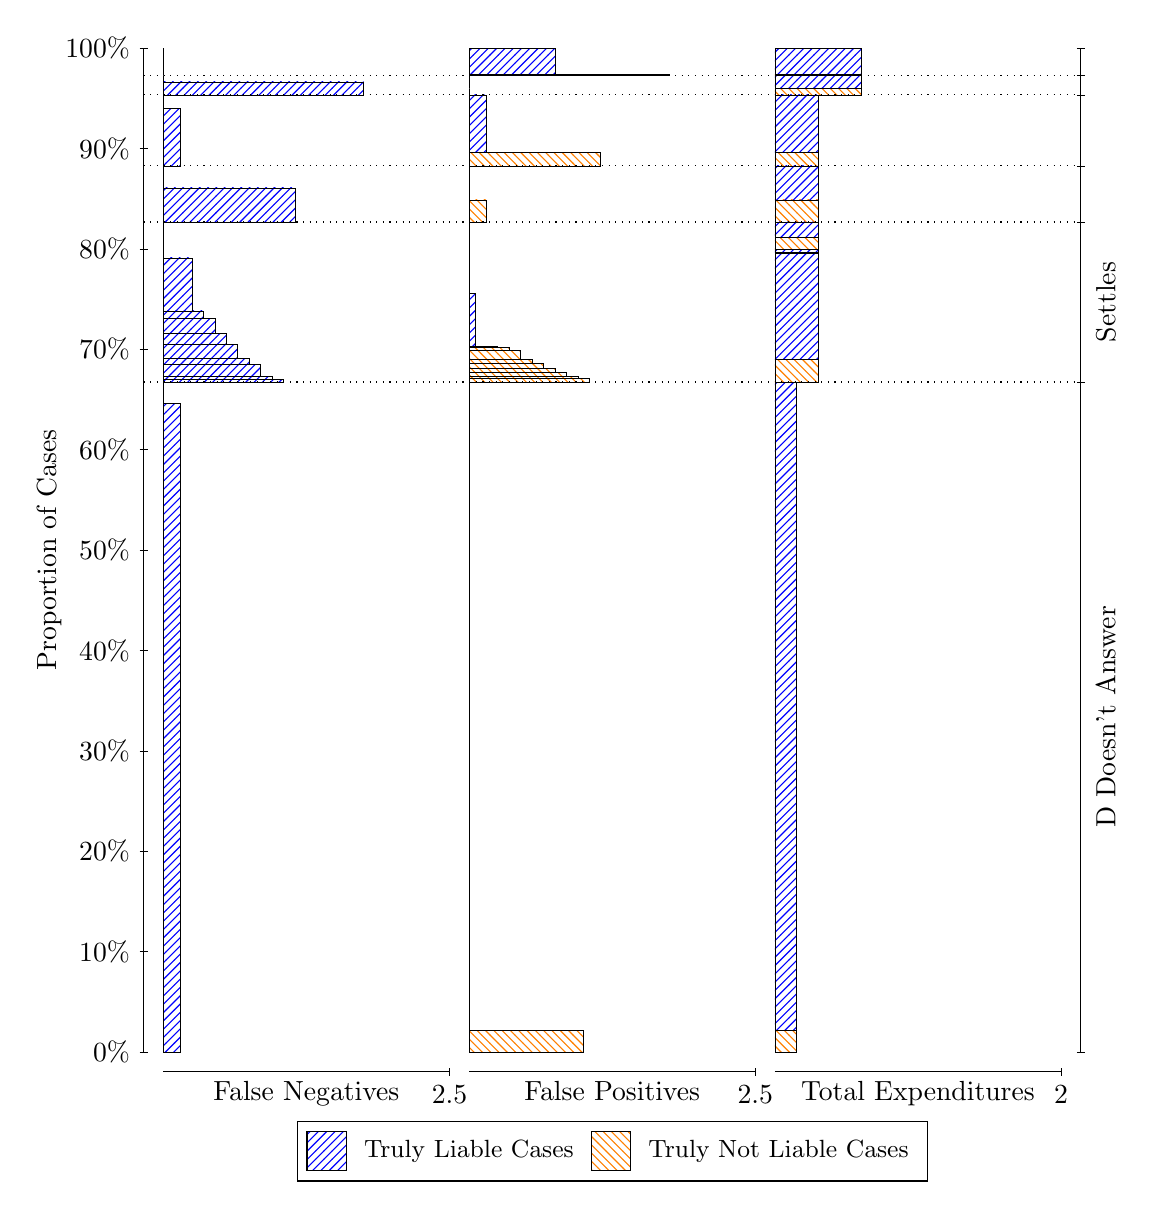
\begin{tikzpicture}
\draw[black, very thin] (1.5,1.75) -- (1.5,14.5);
\node[rotate=90, text=black, anchor=center] at (0.3, 8.125) {Proportion of Cases};
\draw[black, very thin] (1.45,1.75) -- (1.55,1.75);
\node[text=black, anchor=east] at (1.45, 1.75) {0\%};
\draw[black, very thin] (1.45,3.025) -- (1.55,3.025);
\node[text=black, anchor=east] at (1.45, 3.025) {10\%};
\draw[black, very thin] (1.45,4.3) -- (1.55,4.3);
\node[text=black, anchor=east] at (1.45, 4.3) {20\%};
\draw[black, very thin] (1.45,5.575) -- (1.55,5.575);
\node[text=black, anchor=east] at (1.45, 5.575) {30\%};
\draw[black, very thin] (1.45,6.85) -- (1.55,6.85);
\node[text=black, anchor=east] at (1.45, 6.85) {40\%};
\draw[black, very thin] (1.45,8.125) -- (1.55,8.125);
\node[text=black, anchor=east] at (1.45, 8.125) {50\%};
\draw[black, very thin] (1.45,9.4) -- (1.55,9.4);
\node[text=black, anchor=east] at (1.45, 9.4) {60\%};
\draw[black, very thin] (1.45,10.675) -- (1.55,10.675);
\node[text=black, anchor=east] at (1.45, 10.675) {70\%};
\draw[black, very thin] (1.45,11.95) -- (1.55,11.95);
\node[text=black, anchor=east] at (1.45, 11.95) {80\%};
\draw[black, very thin] (1.45,13.225) -- (1.55,13.225);
\node[text=black, anchor=east] at (1.45, 13.225) {90\%};
\draw[black, very thin] (1.45,14.5) -- (1.55,14.5);
\node[text=black, anchor=east] at (1.45, 14.5) {100\%};

\draw[black, very thin] (13.4,1.75) -- (13.4,14.5);
\draw[black, very thin] (13.35,1.75) -- (13.45,1.75);
\node[anchor=west] at (13.35, 1.75) {};
\draw[black, very thin] (13.35,10.258) -- (13.45,10.258);
\node[anchor=west] at (13.35, 10.258) {};
\draw[black, very thin] (13.35,12.291) -- (13.45,12.291);
\node[anchor=west] at (13.35, 12.291) {};
\draw[black, very thin] (13.35,13.004) -- (13.45,13.004);
\node[anchor=west] at (13.35, 13.004) {};
\draw[black, very thin] (13.35,13.906) -- (13.45,13.906);
\node[anchor=west] at (13.35, 13.906) {};
\draw[black, very thin] (13.35,14.15) -- (13.45,14.15);
\node[anchor=west] at (13.35, 14.15) {};
\draw[black, very thin] (13.35,14.5) -- (13.45,14.5);
\node[anchor=west] at (13.35, 14.5) {};

\draw[black, very thin, pattern color=blue, pattern=north east lines] (1.75,1.75) rectangle (1.968,9.987);
\draw[black, very thin, pattern color=orange, pattern=north west lines] (1.75,9.987) rectangle (1.75,10.258);
\draw[black, very thin, pattern color=blue, pattern=north east lines] (1.75,10.258) rectangle (3.276,10.288);
\draw[black, very thin, pattern color=blue, pattern=north east lines] (1.75,10.288) rectangle (3.1307,10.331);
\draw[black, very thin, pattern color=blue, pattern=north east lines] (1.75,10.331) rectangle (2.9853,10.478);
\draw[black, very thin, pattern color=blue, pattern=north east lines] (1.75,10.478) rectangle (2.84,10.561);
\draw[black, very thin, pattern color=blue, pattern=north east lines] (1.75,10.561) rectangle (2.6947,10.732);
\draw[black, very thin, pattern color=blue, pattern=north east lines] (1.75,10.732) rectangle (2.5493,10.874);
\draw[black, very thin, pattern color=blue, pattern=north east lines] (1.75,10.874) rectangle (2.404,11.062);
\draw[black, very thin, pattern color=blue, pattern=north east lines] (1.75,11.062) rectangle (2.2587,11.161);
\draw[black, very thin, pattern color=blue, pattern=north east lines] (1.75,11.161) rectangle (2.1133,11.834);
\draw[black, very thin, pattern color=orange, pattern=north west lines] (1.75,11.834) rectangle (1.75,12.291);
\draw[black, very thin, pattern color=blue, pattern=north east lines] (1.75,12.291) rectangle (3.4213,12.724);
\draw[black, very thin, pattern color=orange, pattern=north west lines] (1.75,12.724) rectangle (1.75,13.004);
\draw[black, very thin, pattern color=blue, pattern=north east lines] (1.75,13.004) rectangle (1.968,13.737);
\draw[black, very thin, pattern color=orange, pattern=north west lines] (1.75,13.737) rectangle (1.75,13.906);
\draw[black, very thin, pattern color=blue, pattern=north east lines] (1.75,13.906) rectangle (4.2933,14.07);
\draw[black, very thin, pattern color=orange, pattern=north west lines] (1.75,14.07) rectangle (1.75,14.15);
\draw[black, very thin, pattern color=orange, pattern=north west lines] (1.75,14.15) rectangle (1.75,14.168);
\draw[black, very thin, pattern color=blue, pattern=north east lines] (1.75,14.168) rectangle (1.75,14.5);
\draw[black, very thin, pattern color=orange, pattern=north west lines] (5.6333,1.75) rectangle (7.0867,2.0207);
\draw[black, very thin, pattern color=blue, pattern=north east lines] (5.6333,2.0207) rectangle (5.6333,10.258);
\draw[black, very thin, pattern color=orange, pattern=north west lines] (5.6333,10.258) rectangle (7.1593,10.307);
\draw[black, very thin, pattern color=orange, pattern=north west lines] (5.6333,10.307) rectangle (7.014,10.334);
\draw[black, very thin, pattern color=orange, pattern=north west lines] (5.6333,10.334) rectangle (6.8687,10.382);
\draw[black, very thin, pattern color=orange, pattern=north west lines] (5.6333,10.382) rectangle (6.7233,10.433);
\draw[black, very thin, pattern color=orange, pattern=north west lines] (5.6333,10.433) rectangle (6.578,10.499);
\draw[black, very thin, pattern color=orange, pattern=north west lines] (5.6333,10.499) rectangle (6.4327,10.542);
\draw[black, very thin, pattern color=orange, pattern=north west lines] (5.6333,10.542) rectangle (6.4327,10.546);
\draw[black, very thin, pattern color=orange, pattern=north west lines] (5.6333,10.546) rectangle (6.2873,10.664);
\draw[black, very thin, pattern color=orange, pattern=north west lines] (5.6333,10.664) rectangle (6.142,10.695);
\draw[black, very thin, pattern color=orange, pattern=north west lines] (5.6333,10.695) rectangle (5.9967,10.715);
\draw[black, very thin, pattern color=blue, pattern=north east lines] (5.6333,10.715) rectangle (5.706,11.388);
\draw[black, very thin, pattern color=blue, pattern=north east lines] (5.6333,11.388) rectangle (5.6333,12.291);
\draw[black, very thin, pattern color=orange, pattern=north west lines] (5.6333,12.291) rectangle (5.8513,12.572);
\draw[black, very thin, pattern color=blue, pattern=north east lines] (5.6333,12.572) rectangle (5.6333,13.004);
\draw[black, very thin, pattern color=orange, pattern=north west lines] (5.6333,13.004) rectangle (7.3047,13.173);
\draw[black, very thin, pattern color=blue, pattern=north east lines] (5.6333,13.173) rectangle (5.8513,13.906);
\draw[black, very thin, pattern color=orange, pattern=north west lines] (5.6333,13.906) rectangle (5.6333,13.986);
\draw[black, very thin, pattern color=blue, pattern=north east lines] (5.6333,13.986) rectangle (5.6333,14.15);
\draw[black, very thin, pattern color=orange, pattern=north west lines] (5.6333,14.15) rectangle (8.1767,14.168);
\draw[black, very thin, pattern color=blue, pattern=north east lines] (5.6333,14.168) rectangle (6.7233,14.5);
\draw[black, very thin, pattern color=orange, pattern=north west lines] (9.5167,1.75) rectangle (9.7892,2.0207);
\draw[black, very thin, pattern color=blue, pattern=north east lines] (9.5167,2.0207) rectangle (9.7892,10.258);
\draw[black, very thin, pattern color=orange, pattern=north west lines] (9.5167,10.258) rectangle (10.062,10.542);
\draw[black, very thin, pattern color=blue, pattern=north east lines] (9.5167,10.542) rectangle (10.062,11.888);
\draw[black, very thin, pattern color=orange, pattern=north west lines] (9.5167,11.888) rectangle (10.062,11.908);
\draw[black, very thin, pattern color=blue, pattern=north east lines] (9.5167,11.908) rectangle (10.062,11.938);
\draw[black, very thin, pattern color=orange, pattern=north west lines] (9.5167,11.938) rectangle (10.062,12.091);
\draw[black, very thin, pattern color=blue, pattern=north east lines] (9.5167,12.091) rectangle (10.062,12.291);
\draw[black, very thin, pattern color=orange, pattern=north west lines] (9.5167,12.291) rectangle (10.062,12.572);
\draw[black, very thin, pattern color=blue, pattern=north east lines] (9.5167,12.572) rectangle (10.062,13.004);
\draw[black, very thin, pattern color=orange, pattern=north west lines] (9.5167,13.004) rectangle (10.062,13.173);
\draw[black, very thin, pattern color=blue, pattern=north east lines] (9.5167,13.173) rectangle (10.062,13.906);
\draw[black, very thin, pattern color=orange, pattern=north west lines] (9.5167,13.906) rectangle (10.607,13.986);
\draw[black, very thin, pattern color=blue, pattern=north east lines] (9.5167,13.986) rectangle (10.607,14.15);
\draw[black, very thin, pattern color=orange, pattern=north west lines] (9.5167,14.15) rectangle (10.607,14.168);
\draw[black, very thin, pattern color=blue, pattern=north east lines] (9.5167,14.168) rectangle (10.607,14.5);
\draw[black, dotted] (1.5,10.258) -- (13.4,10.258);
\draw[black, dotted] (1.5,12.291) -- (13.4,12.291);
\draw[black, dotted] (1.5,13.004) -- (13.4,13.004);
\draw[black, dotted] (1.5,13.906) -- (13.4,13.906);
\draw[black, dotted] (1.5,14.15) -- (13.4,14.15);
\draw[black, very thin] (1.75,1.5) -- (5.3833,1.5);
\node[text=black, anchor=north] at (3.5667, 1.5) {False Negatives};
\draw[black, very thin] (5.3833,1.45) -- (5.3833,1.55);
\node[text=black, anchor=north] at (5.3833, 1.45) {2.5};

\draw[black, very thin] (5.6333,1.5) -- (9.2667,1.5);
\node[text=black, anchor=north] at (7.45, 1.5) {False Positives};
\draw[black, very thin] (9.2667,1.45) -- (9.2667,1.55);
\node[text=black, anchor=north] at (9.2667, 1.45) {2.5};

\draw[black, very thin] (9.5167,1.5) -- (13.15,1.5);
\node[text=black, anchor=north] at (11.333, 1.5) {Total Expenditures};
\draw[black, very thin] (13.15,1.45) -- (13.15,1.55);
\node[text=black, anchor=north] at (13.15, 1.45) {2};

\node[text=black, centered, rotate=90] at (13.72, 6.0038) {D Doesn't Answer};
\node[text=black, centered, rotate=90] at (13.72, 11.274) {Settles};





\draw (7.449999999999999,1.5) node[draw=none] (baseCoordinate) {};
\begin{scope}[align=center]
        \matrix[scale=0.5, draw=black, below=0.5cm of baseCoordinate, nodes={draw}, column sep=0.1cm]{
            \node[rectangle, draw, minimum width=0.5cm, minimum height=0.5cm, pattern color=blue, pattern=north east lines] {}; &
            \node[draw=none, font=\small, text=black] (B) {Truly Liable Cases}; &
            \node[rectangle, draw, minimum width=0.5cm, minimum height=0.5cm, pattern color=orange, pattern=north west lines] {}; &
            \node[draw=none, font=\small, text=black] (B) {Truly Not Liable Cases}; \\
            };
\end{scope}

\end{tikzpicture}
\end{document}